\documentclass[conference]{IEEEtran}
\usepackage[T1]{fontenc}
\usepackage{times}
\usepackage{amsmath,amssymb,graphicx,booktabs}
\usepackage{multicol}
\usepackage[numbers,sort&compress]{natbib}
\usepackage[hidelinks]{hyperref}
\hypersetup{pdfauthor={},pdfcreator={},pdfproducer={},pdftitle={When Does Physical Diagnosis Compromise Robot Recovery?},pdfsubject={Anonymous manuscript}}
\newcommand{\K}{\mathcal K}
\newcommand{\A}{\mathcal A}
\newcommand{\B}{\mathcal B}
\newcommand{\E}{\mathbb E}
\newcommand{\ind}{\mathbb I}
\begin{document}
\title{When Does Physical Diagnosis Compromise Robot Recovery?}
\author{Author Names Omitted for Anonymous Review}
\maketitle
\begin{abstract}
A diagnostic contact can reveal why a manipulation failed while destroying an otherwise available correction. How frequently does this happen beyond the effect of waiting, and does anticipating it improve recovery? We study \emph{post-diagnosis recoverability}: which fixed feedback corrections still complete the task within a common deadline. Matched probe and equal-duration hold executions separate changes caused by contact from lost time, while controlled diagnostic-response tests measure information gained. We formulate two falsifiable hypotheses for contact-rich assembly. H1 predicts at least 10\% constraint-compliant loss of the entire declared recovery repertoire under a frozen information-seeking policy, together with positive diagnostic signal; a secondary test examines their co-occurrence. H2 predicts at least five percentage points higher task completion for recoverability-aware diagnosis under matched constraints and observations. We provide exact finite-model analysis, a fully specified simulation protocol, and an interpretation of positive and null outcomes. The physical hypotheses remain prospective; the contribution is a recovery-specific measurement and decision methodology, not a new contingent-planning solver.
\end{abstract}

\section{Introduction}
A peg has stalled against a fixture. An axial preload or lateral dither might reveal the cause, but the same contact can change what a subsequent correction can accomplish. More accurate diagnosis is of little help if the robot no longer has time, clearance, or a suitable corrective policy to finish. Waiting can remove opportunities too. An experiment must distinguish the physical effect of diagnosis from the effect of its duration.

We ask: \emph{under which post-failure contact conditions does informative diagnosis remove recovery opportunities beyond elapsed time, and when does accounting for those opportunities improve completion?} Recovery is relative to a task, policy catalogue and remaining budget. Losing one correction need not erase the catalogue; staying within physical constraints need not preserve a successful correction.

\begin{figure}[t]
\centering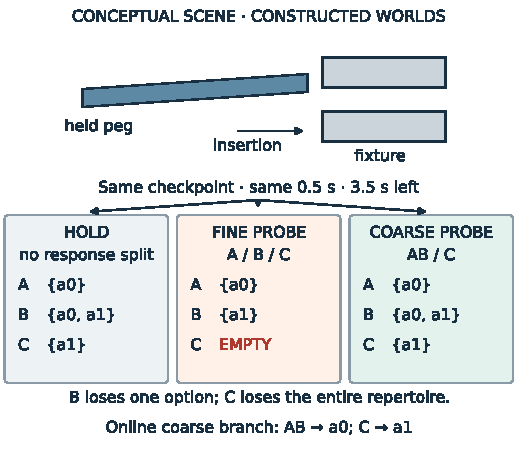
\includegraphics[width=\columnwidth]{figures/figure1.pdf}
\caption{A probe changes both knowledge and the physical state for recovery. In these \emph{constructed worlds} (not robot measurements), equal-duration fine diagnosis identifies A/B/C but destroys C's only successful correction; coarse diagnosis reveals less yet retains a response-dependent correction. The assembly sketch is conceptual. Alternative branches are evaluated offline; only one is executed online.}
\label{fig:thesis}
\end{figure}

Interaction as sensing is established \citep{bohg2017}. s-FEAST couples active fault estimation and probabilistic state constraints \citep{ragan2024}; DA-GRD seeks grasp-relevant agreement while considering contact-induced motion \citep{wang2026}. Reversibility-aware methods \citep{eysenbach2018,grinsztajn2021} and task-compatible calibration's distinction between identifiability and downstream controllability \citep{kobayashi2026} precede this work. Contingent and reach-avoid planning can represent terminal task feasibility \citep{sheng2024}. We do not propose a new POMDP solver or claim these methods cannot express our objective.

We develop a \emph{post-failure measurement and decision methodology} with three linked elements: an operational set of successful remaining corrections, a matched physical probe-versus-hold contrast, and a shared-model comparison of information-seeking and recoverability-aware decisions. The matched contrast identifies what a diagnostic interaction changes beyond elapsed time. The policy comparison asks whether that change actually matters for task completion. Together they turn a familiar possibility, that sensing can disturb objects, into a measurable and falsifiable robotics question.

\textbf{H1: Material physical tradeoff.} A frozen information-seeking probe policy causes full-repertoire erasure, beyond equal-duration holding and on compliant paths, in at least 10\% of eligible checkpoints. Its responses also yield positive population diagnostic signal relative to both the initial observation and holding; erasure-case signal is tested separately.

\textbf{H2: Decision consequence.} A recoverability-aware selector improves task completion by at least five percentage points relative to constrained information seeking, with no more than two points additional measured constraint violations. These are prespecified materiality thresholds, not observed effect sizes.

\section{Recovery Sets and Contingent Decisions}
State $s$ includes physical state, controller memory, completion flag and clock; $h$ is legitimate observation history and $\tau$ remaining time. Fix two executable feedback policies $\A=\{a_0,a_1\}$. Let $G(s,a,\tau)$ be binary completion within $\tau$ under the declared goal, deterministic in the reference model. Define
\begin{equation}
\begin{split}
\K_\tau(s)&=\{a\in\A:G(s,a,\tau)=1\},\\
\operatorname{Common}_\tau(\B)&=\bigcap_{s\in\B}\K_\tau(s).
\end{split}
\label{eq:sets}
\end{equation}
An empty set excludes only these policies within this budget. Nonempty sets for every state in support $\B(h)$ do not imply a common choice. Goal completion alone does not imply path compliance.

Probe $p$ takes $d_p$, follows trajectory $\xi_p(s)$, changes state to $T_p(s)$ and returns $y=O_p(s,T_p(s),\xi_p(s))$. Its nominal support is
\begin{equation}
\B_{p,y}=\{T_p(s):s\in\B(h),\ O_p(s,T_p(s),\xi_p(s))=y\}.
\end{equation}
Recovery starts there with $\tau-d_p$; no within-history reset occurs. For stochastic dynamics use a joint kernel $P_p(ds',dy\mid s)$, including all permitted transitions in robust support. A nominal guarantee does not transfer through physical model mismatch.

For a complete deterministic model with admissible probe and recovery paths, one-probe robust recovery is feasible exactly when
\begin{equation}
\forall\text{ reachable }y:\quad
\operatorname{Common}_{\tau-d_p}(\B_{p,y})\ne\emptyset.\label{eq:criterion}
\end{equation}
The executed correction after $y$ must work for every consistent state, proving necessity; choosing a member of each intersection proves sufficiency. This is ordinary contingent planning. An existing exact implementation and independent policy-tree oracle agree on 1,024 exhaustive small transition, response, recovery and path masks. This verifies nominal logic, not physical prediction.

The prospective recoverability-preserving diagnosis (RPD) selector uses the conventional one-probe value
\begin{equation}
V_p(b,\tau)=\E_y\max_{a\in\A}\E_{s'\mid y,p,b}\widehat G(s',a,\tau-d_p),\label{eq:value}
\end{equation}
comparing probing, direct recovery with full $\tau$, and explicit STOP. STOP ends the attempt and is scored by the completion flag actually measured then, not a fabricated missing rollout. Goal achievement sets an absorbing \emph{task flag}, not a physical reset. Primary validation permits at most one probe.

\section{Separating Physical Loss, Time and Information}
\subsection{Matched physical estimands}
Hold $H_d$ maintains the checkpoint's commanded equilibrium, gains and gripper command for $d=d_p$. Gravity, feedback, contacts and time continue. It is neither frozen state nor a target recentered at every measured pose. Define full-repertoire erasure as
\begin{equation}
L_p=\ind[\K_{\tau-d}(H_d(s))\ne\emptyset\ \land\
\K_{\tau-d}(T_p(s))=\emptyset].\label{eq:loss}
\end{equation}
Report full set differences too: losing $a_0$ while $a_1$ remains is not $L_p$. Also report the secondary compliant-recovery set $\K^C=\{a:G=1,C_a=1\}$. Primary $\K$ is goal-based: an option can reach the goal while violating a recovery-path constraint. With sampled probe/hold compliance $C_p,C_H$,
\begin{equation}
J_p=L_pC_pC_H,\qquad q_{\rm IG}=\E_{D_{\rm eligible}}J_{\pi_{\rm IG}(h)}.
\end{equation}
The selector and predecision eligibility are frozen before confirmation. H1 uses a probe-only IG selector over preload/dither. If neither passes the modeled gate below, it returns $\bot$, with defined policy contributions $J_\bot=D_{0\bot}=D_{H\bot}=0$. These are not physical terminal labels. Report abstention; $q_{\rm IG}$ cannot exceed probe-execution frequency. H2's deployment wrapper can choose direct recovery instead, so H1 is not its unconditional erasure rate. No destructive-best-probe selection, safe-only post-treatment subset or erased-only completion denominator is used.

Matched replay identifies these contrasts only under complete physical/controller replay, source parity and the declared dynamics coupling. Independent pseudorandom parents and within-source stationarity are assumptions, not consequences of hash uniqueness. All branches remain one parent. Repeated noisy rollouts cluster; one failure cannot establish zero stochastic success probability. Scope is repeatability-qualified CPU simulation, not hardware safety.

\subsection{H1: two properties and a co-occurrence diagnostic}
Let $Z$ be the evaluator-only generator mode below. Discovery-frozen predictors $f_0(Z\mid X)$, $f_p(Z\mid X,Y_p)$ and $f_H(Z\mid X,Y_H)$ share a fitting budget. For the frozen selector report
\begin{equation}
D_0=\log f_p(Z)-\log f_0(Z),\quad
D_H=\log f_p(Z)-\log f_H(Z).
\end{equation}
H1 requires a lower bound above $.10$ for $q_{\rm IG}$ and positive lower bounds for both score means. These gains are nats per parent, not automatically mutual information. Erasure and signal could occur on disjoint subsets. Therefore also bound $\E[J_pD_0]$ and $\E[J_pD_H]$ as prespecified secondary diagnostics over \emph{all} parents. Non-erasure rows receive zero weight, not deletion. When $q_{\rm IG}>0$, their signs equal the conditional score means on erasure cases. This checks average co-occurrence for frozen predictors, not informativeness of every erased parent or a refitted subgroup.

For three modes smooth $f\leftarrow(1-3\epsilon)f+\epsilon$, $\epsilon=.001$. All scores and weighted scores lie in $[-b,b]$, $b=-\log\epsilon$. Use the one-sided empirical Bernstein bound \citep{maurer2009}
\begin{equation}
\bar D-\sqrt{2S_D^2\log(2/\alpha)/n}
-14b\log(2/\alpha)/(3(n-1))\label{eq:eb}
\end{equation}
with unbiased variance. H1's three conditions form an intersection--union test, each at $\alpha=.025$. The two secondary weighted-score bounds use $.0125$ each. Abstention-weighted gains describe this diagnostic policy, not a hypothetical response on every root. Broad bounds or uninformative responses leave the mechanism unresolved even if motion damages the task.

For independent eligible binary parents use exact Clopper--Pearson bounds \citep{clopper1934}. At $n=512$, a one-sided $.025$ test against $.10$ rejects from 66 events; binomial-component power at true $.15$ is $.921$. Zero events give a 97.5\% upper bound $.00718$. Attrition changes $n$ and precision; 66 is not a universal threshold or joint H1 power calculation.

\subsection{H2: completion and constraints}
H2 tests $\Delta_U=\E[U(\pi_{\rm RPD})-U(\pi_{\rm IG})]\ge .05$ on the entire eligible confirmation cohort, whether H1 holds or not. Report discordant counts $k_+,k_-$ and concordance $k_0$. For candidate difference $\delta$, the profile log likelihood \citep{wilks1938} is
\begin{equation}
\ell_\delta=\max_q\{k_+\log(q+\delta)+k_-\log q
+k_0\log(1-2q-\delta)\},
\end{equation}
where $q\in[\max(0,-\delta),(1-\delta)/2]$ and $0\log0=0$. The 95\% set has $2(\widehat\ell-\ell_\delta)\le3.841459$; maximize the concave scalar likelihood including boundaries, then bisect endpoints in $[-1,1]$ to $10^{-8}$. Its lower endpoint must exceed $.05$. Below 30 discordances use conservative exact bounds $[L_+-U_-,U_+-L_-]$, with $.0125$ per marginal tail, also reported for every sample. The analogous upper paired bound on violation-risk increase must be below $.02$. Profile coverage is asymptotic. At discordance $.20$ and difference $.10$, normal 95\% half-width is $.0378$, not a power guarantee.

Each primary hypothesis receives one-sided $.025$; H2's two conditions form a conjunction. Primary family control is asymptotic where profile likelihood is used. A profile/exact disagreement is approximate support with unresolved finite-sample sensitivity, not robust confirmation. Other baseline/stratum intervals are descriptive. With $m$ missing paired outcomes, use conservative exact bounds $[L(k_+,n)-U(k_-+m,n),U(k_++m,n)-L(k_-,n)]$ with the same marginal allocation, not a completed-prefix profile. H1 uses $[L(k,n),U(k+m,n)]$. For missing scores, lower the mean to $(\sum D_{\rm obs}-mb)/n$ and bound unbiased variance by $nb^2/(n-1)$ in Eq.~\eqref{eq:eb}; reverse signs for an upper bound. Retain all missing parents; never replace them or infer equality from a degenerate bootstrap.

\section{A Concrete Prospective Assembly Protocol}
The following are \emph{proposed study defaults}, not experimentally qualified settings. Use ManiSkill3 3.0.1/SAPIEN 3.0.3, NumPy 1.26.4, Torch 2.5.1+cpu \citep{tao2025}, PegInsertionSide-v1, panda\_wristcam and CPU PhysX, native 100\,Hz simulation/20\,Hz control. Peg/fixture friction is $.3/.3$ and native finger friction $2/2$, restitution zero. Override \emph{both} episode time-limit wrappers to 200 control ticks: the 30-tick setup plus the 160-tick doubled budget must fit without resetting the elapsed clock. Goal/constraint flags never truncate stepping before the declared deadline; STOP and source failure are separate records. Assembly motivates this setting \citep{tang2023}; no hardware or blocked planner prefix is required.

\subsection{Checkpoint generator and native control}
Native square geometry has $c=3$\,mm per-side clearance, half-length $\ell\sim U[85,125]$\,mm and half-width $r\sim U[15,25]$\,mm. Keep native robot base $(-.615,0,0)$\,m. Place hole frame $H$ at world $(.05,.30,.15)$\,m, identity rotation, compensating its fixture offset; $+x$ is insertion. In $H$, nominal peg centre is $(-2\ell-2c,0,0)$, identity rotation, head $(-\ell-2c,0,0)$. Nominal TCP is $(-2\ell-2c-.060,0,0)$, rotation $R_x(\pi)$; the 60\,mm grasp offset follows the source.

Draw hidden $Z$ uniformly: (i) $y$ offset $\pm1.25c$, $z\sim U[-c/4,c/4]$; (ii) interchange $y,z$; (iii) $y,z\sim U[-c/4,c/4]$, one equiprobable pitch/yaw offset $\pm2\theta_c$, $\theta_c=\arctan(c/(2\ell))$. Signs are independent fair draws; other rotations are zero. Set actual peg centre to nominal centre plus $(0,\delta_y,\delta_z)$ in $H$, and rotation $R_z(\theta_z)R_y(\theta_y)$ about its centre; TCP remains nominal. Thus errors are unknown actual grasp-transform errors, not noise added to exact online object pose. Scales straddle one clearance and comparable tip-angle error, not fitted effects.

Only at initialization, place the peg, set zero body/joint velocities and solve native CPU IK (100 iterations) seeded by task vector $(0,\pi/8,0,-5\pi/8,0,3\pi/4,-\pi/4)$; fingers start at $.04$\,m each. Close for $.5$\,s, then command a $3c$ axial approach in 1\,s. No weld, teleport or reset follows. Use absolute native pd\_ee\_pose, base-frame XYZ Euler angles; arm stiffness/damping/limit are $10^3$\,Nm/rad, $10^2$\,Nm\,s/rad,100\,Nm; gripper values $10^3$\,N/m,$10^2$\,N\,s/m,100\,N, command $-1$. IK must meet $c/10$ Euclidean position and $\theta_c/10$ geodesic rotation residuals. Translation uses $\rho(v)=3v^2-2v^3$, rotation shortest-path interpolation.

Eligibility requires no goal, native two-finger grasp ($.5$\,N, $85^\circ$ defaults), peg--fixture force norm $\ge.5$\,N during the last $.05$\,s, TCP residual $[c/4,4c]$, and the checkpoint constraints below. Root-relative slip starts at zero. For ``RPD-assembly-v1/phase/index/geometry'', take the first four SHA256 bytes big-endian as native reset seed; phases are qual/discovery/confirmation, indices zero-based decimal. Native reset supplies geometry. The full separate ``/fault'' digest seeds NumPy PCG64, drawing $Z$, two fair signs, two transverse uniforms, then an angular-axis bit, consuming unused components too. Check seed uniqueness before collection. Each fixed ID is tried once. Known-ineligible roots and failed sources with UNKNOWN eligibility are distinct dispositions.

\subsection{Actions, observations and measured success}
Let $u_0$ be commanded checkpoint equilibrium. Over $d=.5$\,s, hold keeps $u_0$, preload commands $u_0+(c/2)\rho(k/10)e_x$, dither $u_0+c\sin(2\pi k/10)e_y$, for $k=1,\ldots,10$, setting its last command literally to stored $u_0$. Express offsets in $H$, convert targets to the robot-base frame, and apply by zero-order hold on $[(k-1)/20,k/20)$. Orientation/gripper commands stay fixed. Sample $Y_k$ after that interval's fifth physics substep. Equal final commanded pose need not imply equal physical state. All phases use endpoint-inclusive commands. Remaining $\tau=4$\,s gives 70 recovery updates after ten diagnostic updates.

Write $E=T_C^{-1}T_P$ for peg-in-TCP transform. Policy $a_0$ uses nominal $E$; $a_1$ uses a discovery-trained estimate $\widehat E(X)$ computed \emph{once at the root and held identical across probe/hold/direct branches}. Responses choose a macro, not its parameters. For desired peg pose $P^*$, command TCP $C^*=P^*E^{-1}$. Policy $a_0$ inserts to head $(-.010,0,0)$\,m, peg rotation identity, in 40 updates, then holds. Policy $a_1$ withdraws measured macro-start TCP by $4c$ along $-x$ without rotation in ten; realigns to peg-head $(-\ell-2c,0,0)$, identity rotation, in ten; inserts to the same final target in forty; then holds. Segments start at the preceding commanded endpoint, except the first at measured TCP. Native action updates continue, without extra controller reset, state restore or clock reset.

Primary success is \emph{held stable mid-depth insertion}: head $x\in[-15,15]$\,mm, peg-centre $|y|,|z|\le c/2$, rotation geodesic error $\le\theta_c$, linear speed $\le c$/s and angular speed $\le\theta_c$/s on 26 consecutive 100\,Hz samples spanning $.25$\,s. The evaluator sets an absorbing completion flag but continues monitoring to deadline. This is not released full assembly. The stock head-only event is secondary; historical outcomes remain untouched.

At 100\,Hz check native joint limits, $\|\dot q\|_\infty\le2$\,rad/s, TCP residual $\le4c$, relative-grasp slip $\|\operatorname{trans}(E_0^{-1}E_t)\|\le c$ and rotation geodesic $\le2\theta_c$, and peg--fixture net-force norm $\le10m_{\rm peg}g$. Non-finger robot contact with peg/fixture above $.5$\,N violates the envelope. $C_p,C_H$ cover root to $d$, $C_a$ the macro, and H2 violations the whole post-root attempt. These are sampled constraints, not hardware guarantees. Native impulses/timestep supply \emph{evaluator-only} forces; the monitor provides no privileged corrective feedback. Report path length, commanded motion and time; unavailable effort stays missing.

Online $X$ is 28 scalars: seven arm positions and velocities, TCP position and rotation logarithm relative to nominal, commanded position and rotation logarithm, and $\ell,r$. Fixture/grasp calibration is public. Each $Y_k$ has 23 scalars: seven positions/velocities, TCP position/rotation-log and position residual, hence $d_Y=230$. True peg pose, grasp error, $Z$, contacts and alternative outcomes are evaluator-only. Known fixture geometry does not reveal actual grasp error. No force/aperture sensor is invented.

\subsection{One shared finite model and strong controls}
First screen discovery roots and fit only the root grasp estimator from their evaluator-labeled $T_C^{-1}T_P$. Normalize positions/dimensions by $c$, rotations by $\theta_c$, joint angles/rates by 1\,rad and 1\,rad/s; centre/scale by discovery standard deviation floored at 1. TCP/command positions are expressed in $H$; rotation logarithms are relative to nominal TCP rotation, with principal angle in $[0,\pi]$. Root weights are $w_i\propto\exp[-\|X-X_i\|^2/(2d_X)]$. Estimate translation by weighted mean and rotation by normalized weighted quaternion mean, signs aligned with the first ID; norm below $10^{-8}$ uses that ID's rotation. Freeze before recovery-label collection. Discovery supervision is shared model construction, never test-time oracle access. Estimation is fixed in the physical-loss contrast.

Collect all discovery action labels with that frozen estimator, then fit the observation/outcome model. For probe codewords $Y_{jp}$, channel $P_p(j\mid i)\propto\exp[-\|Y_{jp}-Y_{ip}\|^2/(2d_Y)]$, normalized over $j$. Map a response to nearest codeword, ties by ID; Bayes weights give the smoothed predictors. Hold uses its own equal-budget channel. Per-particle $\widehat G_i(p,a)$ is well defined because recovery parameters do not depend on response codeword $j$. No confirmation labels are fitted.

IG maximizes exact finite-channel information about $Z$; RPD maximizes Eq.~\eqref{eq:value}. They share the expected-success recovery rule and probe gate $\sum_iw_i(1-C_{ip})\le.02$, for \emph{pre-recovery} modeled violations only. H2's IG wrapper uses a common direct action, meaning $\widehat G_i(\mathrm{root},a)=1$ for every positive-weight particle; otherwise H1's probe selector, falling back to best direct expected success on abstention. Direct policy uses that root argmax, so one shared direct rollout suffices. Zero modeled recovery chance selects shorter-duration STOP, scored from the prefix flag. RPD compares direct, probes and STOP. Bayesian task-consensus maximizes expected successful-action coverage with identical transitions, algebraically equaling RPD; this adaptation is not DA-GRD reproduction. Independent response-wise enumeration is an exact equality control. Ties prefer shorter time, smaller commanded path, then ID. Report model errors; discovery particles do not establish complete physical support or calibrated safety.

Before discovery, a 12-candidate qualification pilot uses nominal $E$ for both bootstrap routines and $a_0$ as direct control: seven branches plus repeats for the first two eligible IDs, at most 98 terminal episodes/three worker-hours. It tests execution, not final-policy performance. Require eight eligible roots and complete finite traces, commands/clocks and goals reproducible to $10^{-5}$\,m/$10^{-4}$\,rad. Regenerate initialization and the 30-tick prefix in fresh processes; do not trust ordinary snapshots. Check body/joint state, drive targets, command, estimator, absolute clock and dwell memory. After fitting the final estimator, repeat all eight branches for the first two eligible retained discovery IDs (16 episodes) before confirmation. Root failures are attrition; branch violations and failed goals stay measured outcomes, not source exclusions. No gate uses erasure, accuracy or advantage. Source failure stops without task/parameter search. These pilots have not run.

\section{Fixed Validation and Interpretable Outcomes}
Use 64 discovery and 512 confirmation candidates in disjoint phases. Discovery must supply at least two eligible roots and complete paired labels for every retained particle; otherwise the model is unavailable, without outcome imputation. Freeze models/policies before confirmation. Finish its entire eligibility screen before terminal comparisons. UNKNOWN eligibility prevents an unconditional eligible-population claim; any source-evaluable restriction must be reported. Every known eligible parent, including missing, unsafe, uninformative and non-erasing branches, remains in the fixed denominator. Effective $n$ may be below 512. Check every regenerated root against its screened fingerprint, not just the two pilot repeats.

With full eligibility, confirmation needs $512\times3\times2=3{,}072$ matched terminal branches plus 512 full-deadline direct-policy branches. Discovery needs $64\times8=512$, including both direct recoveries to model the full-deadline option. Base cost is \textbf{4,096 terminal branches}. Screening adds at most 576 episodes and final-estimator parity 16; observations come from the same rollouts. Branches do not increase $n$. Before confirmation, pilot timings determine only whether this fixed study fits, never its margins. One CPU worker, 60\,s per episode including setup, a 28-worker-hour ceiling (three qualification, twenty primary, five sensitivities), and ascending ID then hold/preload/dither, $a_0/a_1$, then direct define execution order. Finish or mark missing the atomic parent; retain unfinished IDs and full-cohort bounds. Assembly validation remains prospective.

On 64 confirmation IDs selected by hash before outcomes, doubling $\tau$ adds 384 terminal branches. A pre-existing extra skill adds 192 only if named and qualified before confirmation; none is bound, so that sensitivity is unavailable. A response-blind rule fixed from $X$ alone is scored on the same post-probe branches. It measures response decision value without multiple online executions. No hardware campaign is required.

In the constructed uniform A/B/C example, hold/coarse leave $\{a_0\}$, $\{a_0,a_1\}$, $\{a_1\}$; fine leaves $\{a_0\}$, $\{a_1\}$, $\emptyset$. Paths obey the nominal constraints. Fine information is $\log3=1.099$ nats with best completion $2/3$; coarse information is $.637$ nats with completion 1. Task-consensus and full-objective planning tie RPD. This is logical possibility at equal durations, not a physical prevalence or algorithmic-advantage result.

Existing cube source checks comprise 14 valid fresh-process episodes at one inspected parent per task. Pick release histories lose continuation while recovery remains; Push retains both. No full erasure appears in these retrospective contrasts. The preceding pilot crashed after 38 completed branches per task; original lost outcomes remain missing and isolated replay does not establish global stability. Cube neutral commands differ from the proposed equilibrium hold. These checks neither qualify assembly nor test H1/H2.

Support for H1 establishes its two population properties; weighted-score diagnostics additionally address average signal on erasure cases. H2 support establishes its completion margin against IG jointly with constraint noninferiority, not superiority over equivalent task-aware planning. H1 without H2 shows loss without the proposed benefit; H2 without H1 could reflect partial-option changes. Report hold-empty repertoires separately: inadequate skill coverage is not harmless diagnosis. A narrow interval below $.10$ limits this selector's prevalence; uninformative probes and source failure are different outcomes. Recovery at $2\tau$ indicates deadline dependence; an extra skill would indicate catalogue dependence. None licenses effect-rich test selection.

\subsection{What the controls can and cannot identify}
Equal-duration holding controls elapsed time under the same feedback law; it does not make a probe non-disturbing. The common root-frozen estimator prevents a poorer post-probe belief from silently redefining recovery commands. Differences still concern these fixed feedback policies and their interaction with contact and controller state, not all physically possible controllers. Goal-based and compliant-recovery masks distinguish task loss from loss of a constraint-compliant correction. Root parity and continuous clock checks distinguish intervention effects from invalid branch reconstruction.

Response-blind versus response-aware catalogue choice tests telemetry's decision value with execution parameters fixed. The hold predictor tests information beyond waiting. H2 gains can reflect saved probe time or action choice, not mediation by erasure alone. Report descriptive overlap with $J_p$ and compare the same selected macro on paired hold/probe traces; this cross-world evaluator diagnostic is not a deployable policy. Mode prediction does not identify a hidden physical cause, and a lower modeled risk is not calibrated safety.

The 12-parent technical pilot can establish only source availability at its inspected roots; continued per-parent parity is needed. Large UNKNOWN eligibility or outcome missingness can make inference vacuous. The score bounds can also be conservative at rare erasure rates; H1's binomial power does not ensure a decisive co-occurrence test. If the weighted intervals remain broad, the paper must retain the weaker two-population conclusion rather than claim same-case informative erasure. This is an unresolved empirical hypothesis, not an invitation to lower the margin or select different roots.

All assembly settings remain proposed and require bounded source qualification. No assembly outcomes currently establish physical prevalence, diagnostic co-occurrence or completion gain. A qualified simulation study can answer the fixed question without unavailable hardware; transfer to a robot remains outside scope. The commitment is to report information, complete option sets, completion, constraints, attrition and baseline equality together, including a qualified null.

\clearpage\onecolumn
\begin{multicols}{2}
\bibliographystyle{plainnat}
\bibliography{references}
\end{multicols}
\end{document}
